\documentclass{rapportECL}
\usepackage{lipsum}
\usepackage{gensymb}
\usepackage{pdfpages}
\title{Rapport ECL - Template} %Titre du fichier

\begin{document}

%----------- Informations du rapport ---------

\UE{ELC D6 - PLM maquettage numérique} %Nom de la UE
\sujet{Rapport de projet : VBA Lotus - Catia } %Nom du sujet
\titre{EPSA - LASauto (v2)} %Titre du fichier .pdf

\enseignant{Didier \textsc{Lacour}\\
            {Paul \textsc{Clozel}} } %Nom de l'enseignant

\eleves{\textsc{Schio} Michele \\
        \textsc{Matteï} Calixthe} %Nom des élèves

%----------- Initialisation -------------------
        
\fairemarges %Afficher les marges
\fairepagedegarde %Créer la page de garde
\tabledematieres %Créer la table de matières

%------------ Corps du rapport ----------------


\section{Introduction}

\subsection{Contexte et motivation} %------------------------------------------------

\par Lotus est un logiciel d'analyse cinématique de la Liaison Au Sol (LAS) d'une voiture. Il permet notamment de définir les points caractéristiques des liaisons types d'une liaison au sol, de définir ces liaisons et d'étudier leur mouvement.

\par La démarche courante à l'EPSA combine une feuille de calcule Excel avec une génération des pièces par Catalogue CATIA:  cette méthode est très fonctionnelle mais également un peu lente. Une fois la configuration de points déterminée (sur Lotus), il est nécessaire d'ouvrir un tableau Lotus, de sélectionner manuellement les coordonnées des points, les copier-coller sur un fichier Excel dédié au paramétrage, enregistrer et fermer le fichier Excel, ouvrir le Catalog LASauto, ouvrir la fenêtre de mise à jour, sélectionner tous les composants dans l'arbre, lancer la mise à jour, attendre quelques minutes, fermer le Catalog, ouvrir l'assemblage de travail, faire une mise à jour et vérifier que tout s'est bien passé.

\par Ainsi, l'optimisation de la LAS d'un véhicule, typiquement pour un véhicule EPSA, nécessite de nombreuses itérations afin de tendre vers une géométrie et un confinement offrant une dynamique véhicule et un poids optimal. Il est donc primordial pour l'EPSA d'optimiser les mises à jour de LAS afin de gagner un temps considérable. Le but de ce projet est donc de permettre la mise à jour des composants à l'intérieur de l'Assemblage de Liaison au Sol du Véhicule dans Catia (Assemblage qui sera nommé plus tard simplement \texttt{Suspension}), mise à jour possible directement en lançant la Macro, par lecture du fichier Lotus, sans intervention manuelle sur l'Assemblage et sans utiliser la technologie de Catalog. Il est également souhaité de pouvoir définir de façon adaptée les pièces de l'assemblage de travail.

\par L'intérêt de ce rapport est donc de permettre la compréhension du code et de pouvoir utiliser la macro convenablement.


\subsection{Structure d'un fichier Lotus} %-------------------------------
\par Etant donné que ce projet est fondé sur l'étude d'un fichier Lotus au travers d'une macro Catia, la compréhension de la structure d'un tel fichier est importante.
Le fichier d'enregistrement de Lotus est de type \texttt{.dat}. Il s'agit d'un fichier Texte structuré afin de pouvoir enregistrer les différents paramètres d'un modèle Lotus. Le fichier est composé de différentes sections, ayant pour titre : \texttt{VERSION}, \texttt{PARAMETERS}, \texttt{TEMP\_GRAPHICS}, \texttt{TEMP\_SETTINGS}, \texttt{FRONT SUSPENSION}, \texttt{REAR SUSPENSION},
\texttt{COMPLIANCE} et
\texttt{MODAL}. Tout ceci est résumé dans la Fig.\ref{fig:structure_lotus}

\begin{figure}
    \centering
    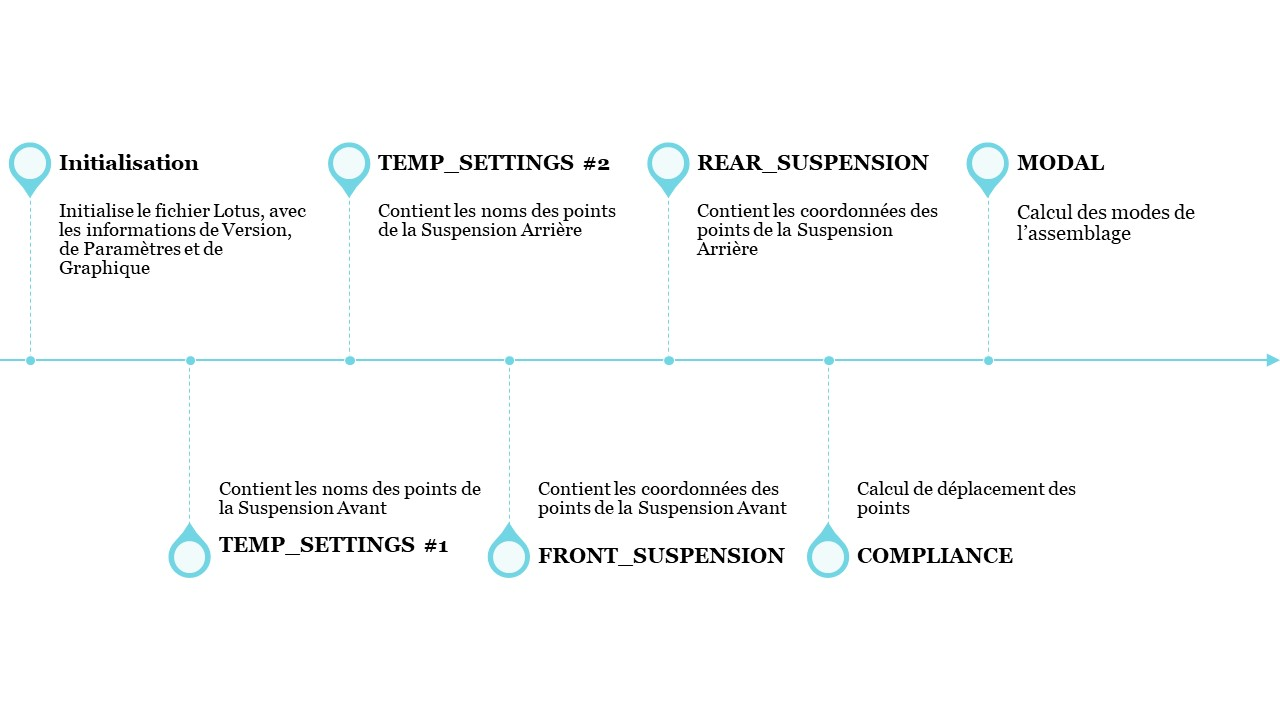
\includegraphics[width=\linewidth]{img/Structure_Fichier_Lotus.jpg}
    \caption{Structure d'un Fichier Lotus}
    \label{fig:structure_lotus}
\end{figure}

\newpage
\par Ainsi, Lotus définit des modèles d'architecture pour différentes géométries de Suspension. Une géométrie de Suspension modifie tout simplement ce modèle et enregistre les nouvelles coordonnées des points dans un fichier \texttt{.dat}. \par Dans la section \texttt{TEMP\_SETTINGS} de ce fichier, on retrouve la définition des pièces de la suspension ainsi qu'une liste des points du modèle de suspension choisi.
\par Dans la section \texttt{FRONT SUSPENSION} et \texttt{REAR SUSPENSION}, on retrouve les coordonnées des points du modèle de suspension (respectivement pour le train avant et arrière).
\par Ce sont ces deux types de sections qui vont nous intéresser.


\paragraph{Structure de la section \texttt{TEMP\_SETTINGS}} %----------------

\par Un exemple de section \texttt{TEMP\_SETTINGS} d'un fichier Lotus est présenté en Fig. \ref{fig:temp_settings}. Après l'entête (ligne 1) et la description du template utilisé pour la création du modèle Lotus (lignes 2 et 3), on retrouve une série de nombres. Le premier indique le nombre de pièces dans le modèle et le deuxième le nombre de points dans le fichier. Dans l'exemple de la Fig. \ref{fig:temp_settings}, le nombre de pièces est 6 et le nombre de points est 2. Le nom de chaque pièce est listé de la ligne 5 à la ligne 10, suivi de la définition de chaque point dans le modèle. On s'intéresse ici seulement à la lecture du nom du point : on lit donc la ligne 11 ( pour le point numéro 1) et on saute 8 lignes pour arriver à la définition du point numéro 2 (ligne 20).

\begin{figure}
    \centering
    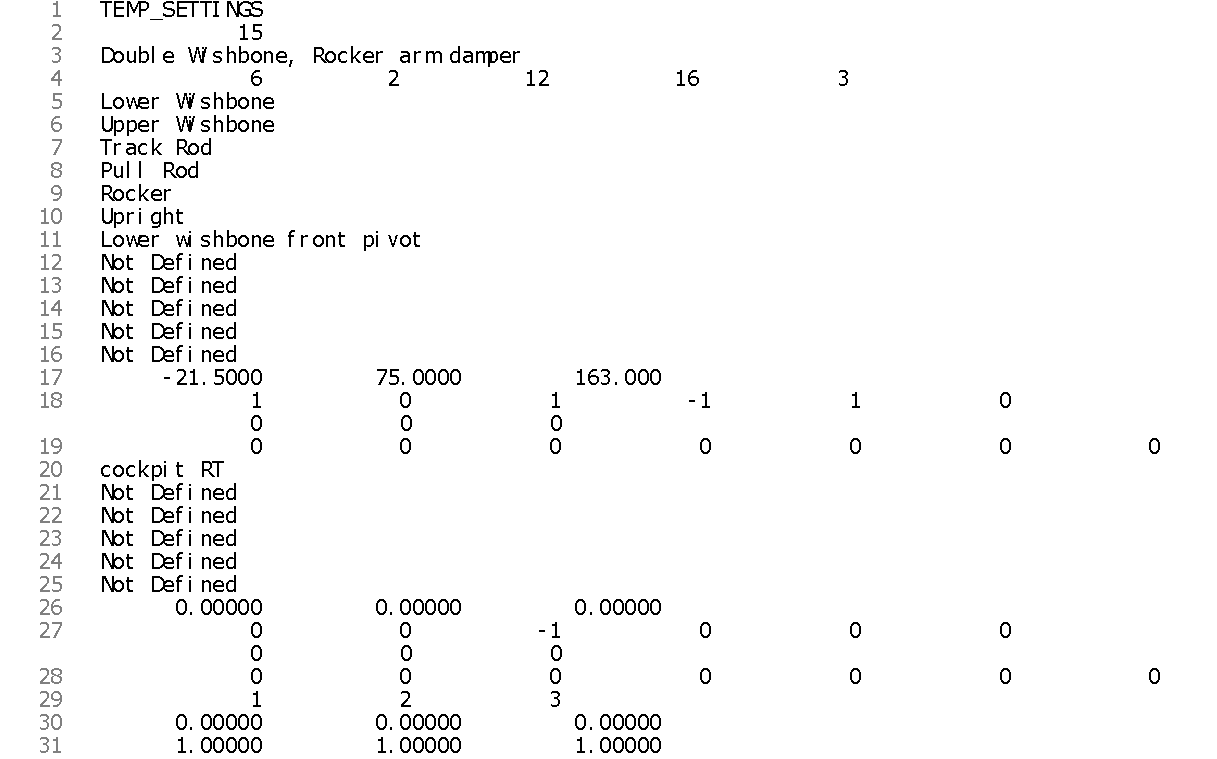
\includegraphics[width=\linewidth]{fichiers/temp_settings.pdf}
    \caption{Structure de la section \texttt{TEMP\_SETTINGS} avec 2 points}
    \label{fig:temp_settings}
\end{figure}


\paragraph{Structure de la section \texttt{FRONT (REAR) SUSPENSION}} %---------------------

\par Un exemple de section \texttt{FRONT SUSPENSION} est présenté en Fig. \ref{fig:frontSuspension}. Après l'entête (ligne 3), on retrouve le code du template utilisé (ligne 2 Fig. \ref{fig:temp_settings}) et ensuite un tableau de coordonnées des points du Template. Cet exemple utilise un Template avec 27 points, les coordonnées sont donc listées dans les lignes 5 - 31

\begin{figure}
    \centering
    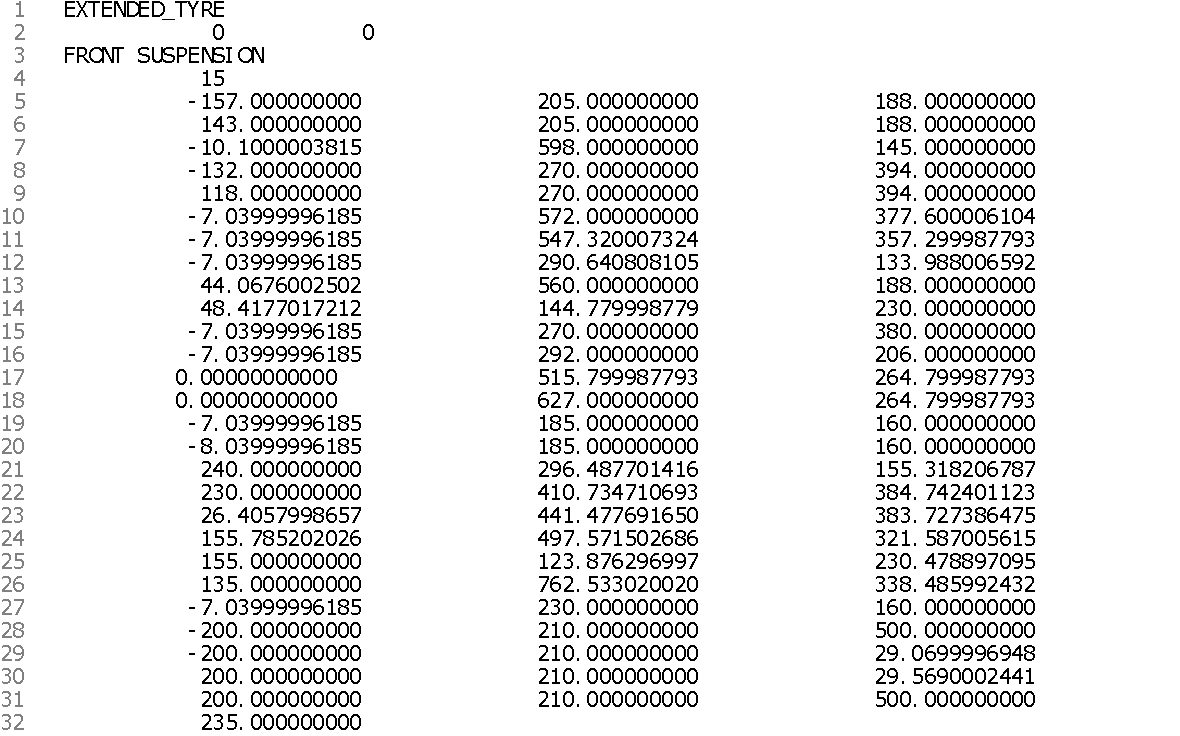
\includegraphics[width=\linewidth]{fichiers/front suspension.pdf}
    \caption{structure de la section \texttt{FRONT SUSPENSION}}
    \label{fig:frontSuspension}
\end{figure}

\newpage
\subsection{Besoins du système LAS vis à vis de la maquette} % ----------------------

\par Les besoins du système liaison au sol sont résumés ci-dessous, représenté par d'abord le pseudo-code de l'application puis le cahier des charges qu'a dû respecter notre application.\\

\paragraph{Pseudo-code}
\noindent\textit{Inputs, obtenu grâce à l'utilisateur, après lancement de l'Userform} (cf Section \ref{interf_graph})
\begin{itemize}
    \item Path du fichier Lotus .dat
    \item Path du Wireframe.CATProduct contenant LotusPoint.CATPart
    \item Paths d'autres Products à mettre à jour
\end{itemize}
\textit{Running}
\begin{itemize}
    \item \textbf{Appel du module LectLotus} (cf Section \ref{lect_lotus}),
        \subitem{- Lecture du fichier .dat}
        \subitem{- Récupération, dans des listes, des noms et des coordonnées des points du train avant et arrière}
    \item \textbf{Appel du module MajCatia} (cf Section \ref{majcatia}),
        \subitem{- Ouverture de fichier LotusPoint.CATPart}
        \subitem{- \textbf{Pour} i=1 à len (nom\_points train avant)}
            \subsubitem{- Si le point existe déjà :}
                \subsubsubitem{Mise à jour de ses coordonnées}
            \subsubitem{- Sinon :}
                    \subsubsubitem{Création du point}
        \subitem{- \textbf{Pour} i=1 à len (nom\_points train arrière)}
            \subsubitem{- Si le point existe déjà :}
                \subsubsubitem{Mise à jour de ses coordonnées}
            \subsubitem{- Sinon :}
                    \subsubsubitem{Création du point}
        \subitem{- Mise à jour de LotusPoints.CATPart}
        \subitem{- Mise à jour de Wireframe\_Definition.CATProduct}
        \subitem{- Mise à jour des autres Products sélectionnées par l'utilisateur}
        \subitem{- Fermeture de tous les fichiers Catia}
\end{itemize}
\textit{Outputs}
\begin{itemize}
    \item Nombre de points créés et mis à jour pour le train avant
    \item Nombre de points créés et mis à jour pour le train arrière
\end{itemize}

\paragraph{Cahier des charges de l'application VBA} %----------------------------

\begin{itemize}
    \item Offrir une interface graphique à l'utilisateur
    \item Permettre à l'utlisateur la sélection, par explorateur de fichiers, des documents qu'ils souhaitent utilisés, mettre à jour, etc
    \item Permettre la lecture des points et leurs coordonnées depuis un fichier Lotus \texttt{.dat} sélectionné à partir de l'explorateur de fichiers
    \item Mettre à jour le fichier Catia automatiquement et d'autres fichiers Catia souhaités par l'utilisateur
    \item Indiquer le nombre d'opérations sur les coordonnées effectuées à l'utilisateur afin qu'il puisse vérifier la bonne exécution du programme
    \item Anticiper quelques erreurs classiques et les indiquer à l'utilisateur quand il les exécute
    \item Pouvoir réutiliser les fichiers de conception détaillée de la saison 2020
\end{itemize}{}
\section{Lecture du fichier Lotus}
\label{lect_lotus}

\subsection{Organisation du code}

La démarche employée a ainsi été de repérer d'abord les deux sections \texttt{TEMP\_SETTINGS} afin de récupérer le nom des points pour créer une liste de noms des points de la Suspension Avant, puis les noms des points de la Suspension Arrière.
\par Ensuite, le code repère la section \texttt{FRONT\_SUSPENSION} et crée la liste des coordonnées des points de la Suspension Avant, et de manière analogue, la liste des coordonnées des points de la Suspension Arrière est créée.

\par Pour résumer, voilà la structure synthétique du code : 

\begin{enumerate}
    \item Ouverture du fichier txt
    \item Lecture des différentes parties de ce document
    \item Sauvegarde des valeurs lues
\end{enumerate}


\subsection{Bibliothèques utilisées }
\paragraph{Gestion des chemins de fichier avec accents}  \texttt{Option Compare text} est une bibliothèque à mettre avant le \texttt{Sub}, car il permet de comparer des chaînes selon un ordre de tri alphabétique en ne tenant pas compte de la casse qui est déterminé par les paramètres régionaux du système informatique utilisé.

\paragraph{TextStream} Bibliothèque VBA permettant de créer un fichier TextStream à partir d'un fichier texte. Ce fichier TextStream permet de nombreuses manipulations sur ses lignes sans se soucier d'interférer ou non sur le fichier original. De plus, cette méthode permet d'avoir un objet à passer aux différentes fonctions pour la lecture du texte. Enfin, une fois ce fichier prêt, il est possible de l'enregistrer en tant que fichier txt final.

\paragraph{Dynamic Arrays} On utilise la méthode \texttt{Dim} - \texttt{ReDim} afin de pouvoir définir une liste et de pouvoir déclarer sa taille réelle en fonction des paramètres lus depuis le fichier Lotus. Il faut faire attention car cette définition se fait en utilisant l'indice de la liste et non sa taille (cf. documentation Microsoft pour \texttt{ReDim})

\paragraph{Conversion de string à double} Le caractère de séparation des décimaux dans Lotus est celui du local anglais (le point). Il se peut que dans l'ordinateur où on exécute la macro, le local soit différent de celui anglais et dans ce cas, la conversion d'une \textit{string} en \textit{double} ne se fait pas correctement. Pour cela, on remplace avec \texttt{replace} le caractère point avec une virgule lors de la lecture des cordonnées dans le tableau Lotus puisque changer le séparateur dans le local de la machine n'est pas conseillé.

\subsection{Lecture du fichier \texttt{.dat}}%-------------------------------------

\par Pour la lecture du morceau de texte présenté en Fig. \ref{fig:temp_settings} voir la Subroutine \texttt{ReadTempSettings} et ses commentaires.
De même pour la lecture du morceau de texte présenté en Fig. \ref{fig:frontSuspension} voir la Subroutine \texttt{ReadSuspension} et ses commentaires.


\section{Mise à jour du produit Catia}
\label{majcatia}

\subsection{Principe de fonctionnement}

\par La Fig. \ref{fig:idea} présente la structure type des fichiers de travail : l'idée est de laisser l'utilisateur définir un filaire \textit{ad hoc} dans le produit \texttt{WireframeDefinition.CATProduct} en créant des pièces (\texttt{Wireframe1.CATPart}, \texttt{Wireframe2.CATPart}, ...) avec des projections des points de \texttt{LotusPoints.CATPart}. La macro fait tout simplement une mise à jour des points dans  \texttt{LotusPoints.CATPart} avec les valeurs lus depuis un fichier \texttt{Lotus.dat} et appelle une mise à jour complète du produit \texttt{WireframeDefinition.CATProduct}. 
\par Etant donné que les points du train avant et arrière ont les mêmes noms, \texttt{LotusPoints.CATPart} contiendra deux corps, permettant ainsi de différencier le train avant et arrière lors de la mise à jour.
\par Ensuite, les pièces filaires (\texttt{Wireframe1.CATPart}, \texttt{Wireframe2.CATPart}, ...) peuvent être mises dans un produit séparé (\texttt{Suspension.CATProduct}) pour la conception détaillée. 

\paragraph{Voici les différents avantages de cette approche:}

\begin{itemize}
    \item définition du filaire \textit{ad hoc} sur un produit dédié : possibilité de définir des nouvelles pièces dans le filaire sans modifier la macro, permettant d'anticiper l'apparition de nouveaux sous-systèmes dans la suspension du véhicule, non présents lors des itérations précédentes (par exemple, ajout d'une barre anti-roulis)
    \item une mise à jour de \texttt{Suspension.CATProduct} ne modifie pas les pièces filaires puisque ces dernières ont été définies dans le contexte de \texttt{WireframeDefinition.CATProduct}: autrement dit la mise à jour des points est indépendante du fichier de conception détaillé
    \item Possibilité d'adapter la construction des pièces filaires aux exigences de forme : placement des repères au centre des pièces
\end{itemize}{}

\begin{figure}
    \centering
    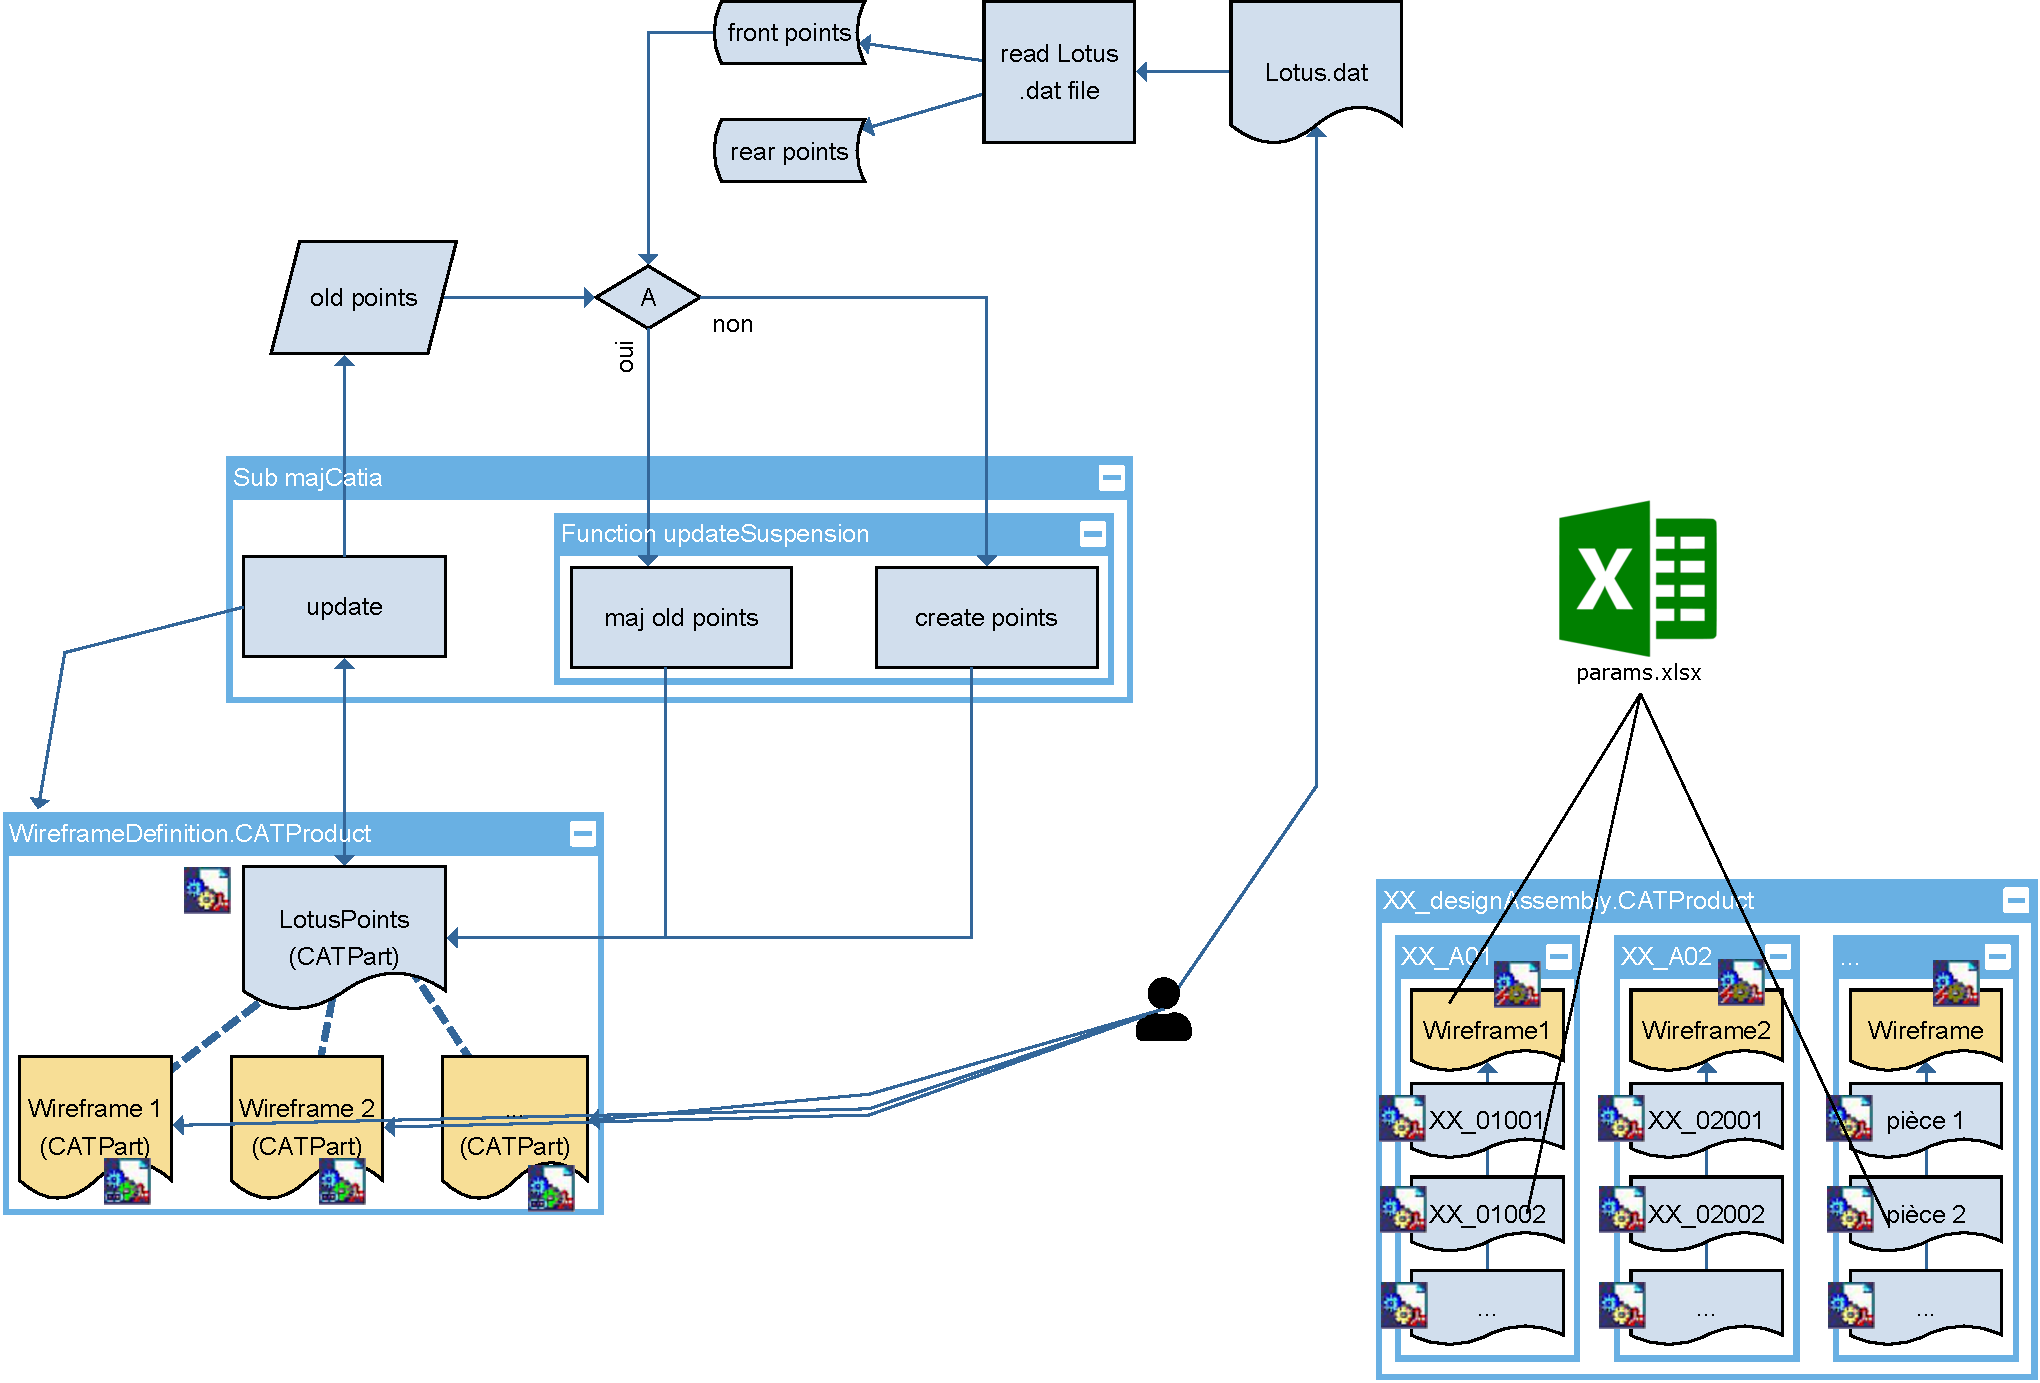
\includegraphics[width=\linewidth]{img/schemaAll.pdf}
    \caption{Représentation schématique du principe de fonctionnement de la macro}
    \label{fig:idea}
\end{figure}

\subsection{Description et organisation du code} %-----------------------------------

\par Dans le module \textit{majCatia}, la subroutine \textit{maj\_Catia} permet de mettre à jour les points présents dans  \texttt{LotusPoints.CATPart} avec les noms et les coordonnées lues depuis le fichier Lotus, comme expliqué dans la section précédente. 

\par Grâce à l'ouverture du produit \texttt{WireframeDefinition.CATProduct}, nous pouvons accéder directement au fichier \texttt{LotusPoints.CATPart}, étant déjà chargé dans la mémoire.
Ainsi, le code fait tout d'abord une scan des points déjà présents dans \texttt{LotusPoints.CATPart} afin de pouvoir distinguer la création d'un nouveau point de la mise à jour d'un point existant. Ensuite, nous faisons une comparaison entre les noms présents dans la liste globale \texttt{frontNames} (créée avec la lecture du ficher Lotus.dat pour le train avant) et \texttt{rearNames} (de manière analogue pour le train arrière) avec ce qui était présent dans les deux corps de \texttt{LotusPoints.CATPart}:
\begin{itemize}
    \item si le point existe déjà, ses coordonnées sont mises à jour en passant par les paramètres de l'objet
    \item sinon, un nouveau point est créé en utilisant la méthode \textit{hybridShapeFactory} et ajouté dans l'arbre de la pièce
\end{itemize}



\par Petit détail concernant la conception à l'EPSA : la conception détaillée est faite par convention sur la partie gauche du véhicule, puis mis en symétrie. Néanmoins, les points Lotus sont définis à droite : nous avons simplement changer le signe de la coordonnée \texttt{Y} afin de réaliser la symétrie.

\subsection{Précautions et points faibles} % ------------------------------------------------------

\par Premièrement, nous remarquons que l'identification des points se base sur leur nom. Pour changer cette propriété, il faut rentrer directement dans le paramétrage du logiciel Lotus. \par On remarque deuxièmement que cette macro ne peut pas effacer des points dans\\ \texttt{LotusPoints.CATPart}. Pour ce faire, il faut ouvrir manuellement la pièce dans Catia et supprimer les point dans l'arbre. L'intérêt de ceci est d'éviter que la macro efface les mauvais points si l'utilisateur n'est pas précautionneux et nomme de la même manière les nouveaux  points et ceux qu'il a supprimé dans Lotus.

\section{Interface Graphique}
\label{interf_graph}
\subsection{Cahier des Charges spécifique} %-------------------------------
\begin{itemize}
    \item Sélection dynamique du fichier Lotus depuis l'explorateur de fichiers puisque ce fichier va changer très souvent (versionnement des fichiers Lotus, donc versionnement de la LAS de le voiture, se fait par enregistrement de différents fichiers) 
    \item Affichage des messages d'erreur et du résumé de mise à jour
    \item Bouton mise à jour de l'assemblage
    \item Sélection dynamique du fichier Catia depuis l'explorateur du fichier : mémoriser le parcours d'enregistrement des fichiers \texttt{WireframeDefinition.CATProduct} car il ne vont pas changer très souvent.
    \item donner la possibilité à l'utilisateur de sélectionner d'autres produits à mettre à jour après la mise à jour des points
    \item Conserver les derniers produits updatés lors de l'itération précédente, afin de faire gagner du temps à l'utilisateur lors des nombreuses itérations.
\end{itemize}


\subsection{Définition de l'interface} %----------------------------------
\begin{minipage}{\textwidth}
    \centering \vspace{1em}
    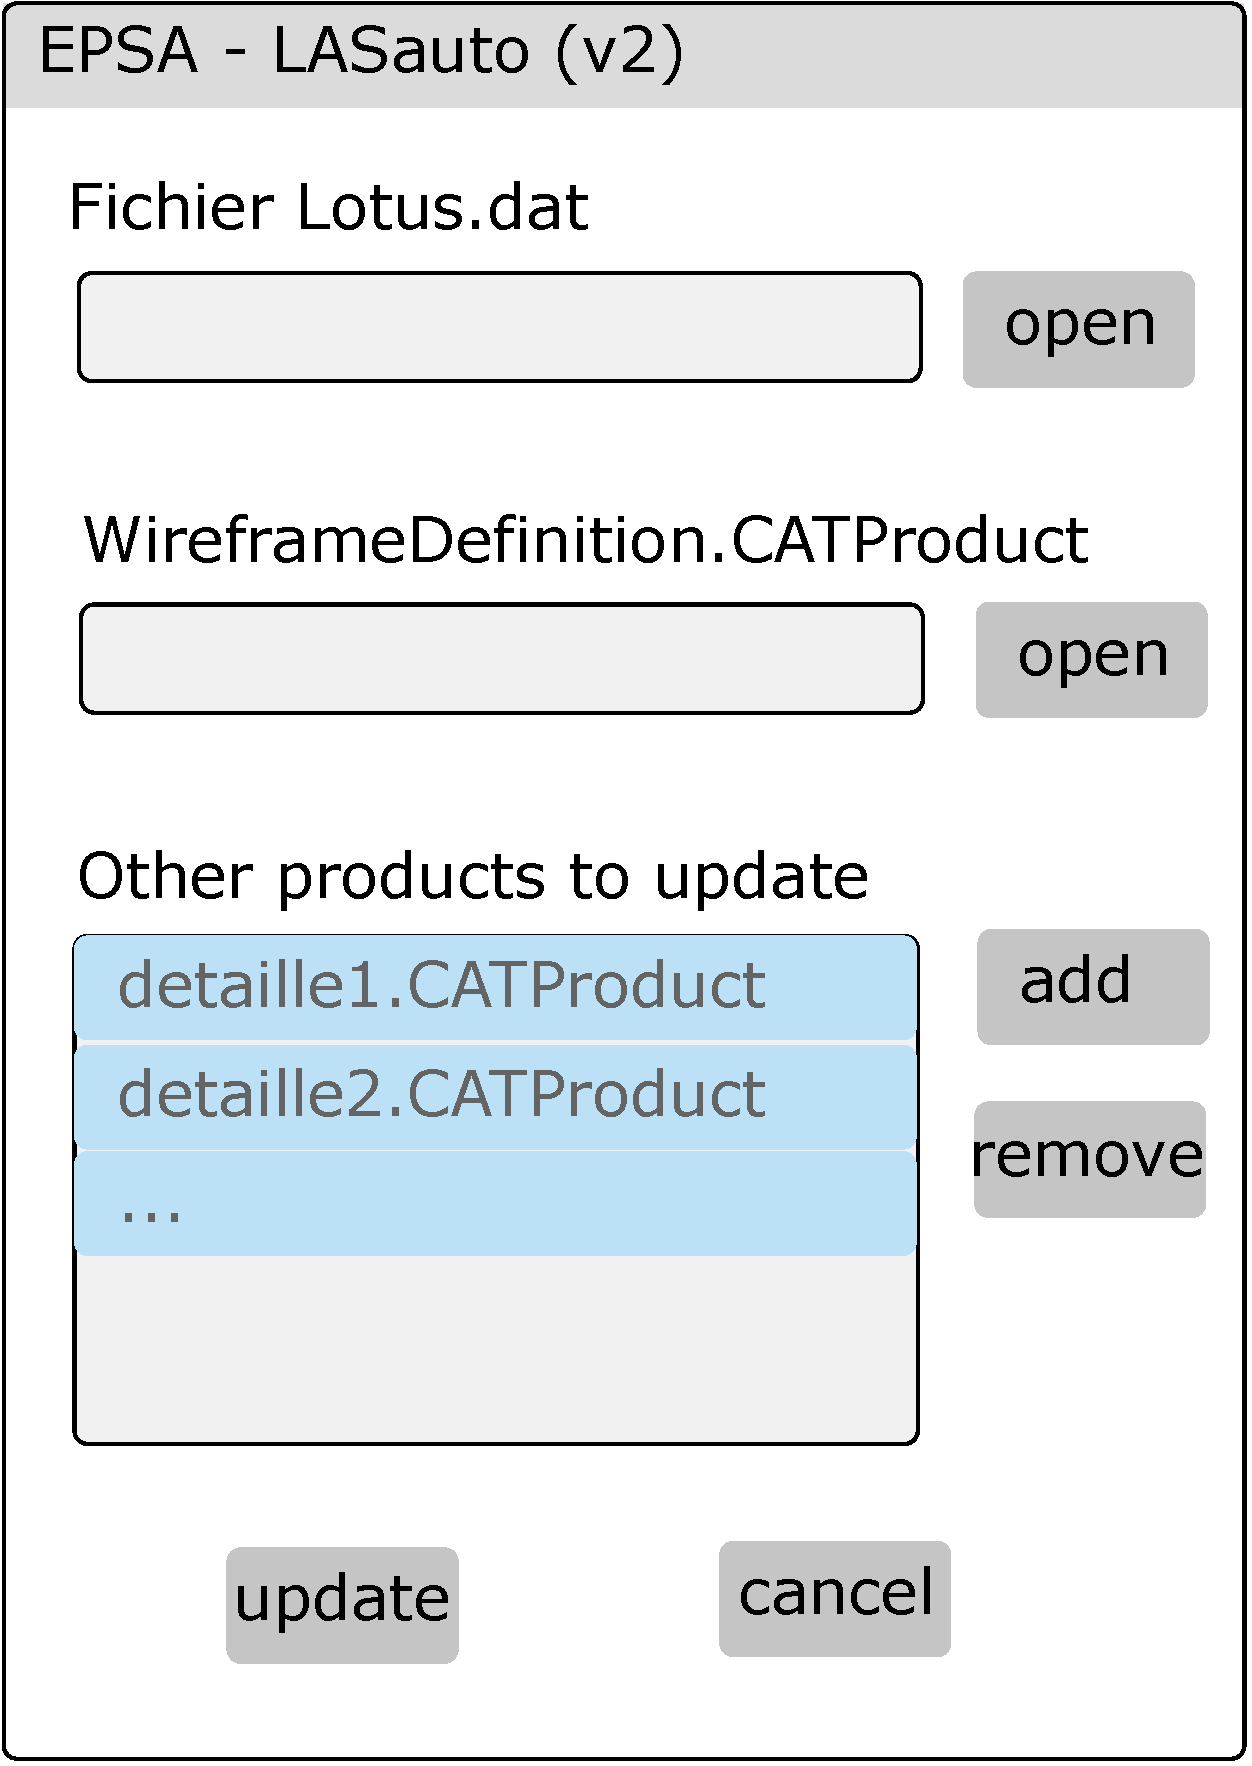
\includegraphics[height=10cm]{img/interfaceGraphique.pdf}
    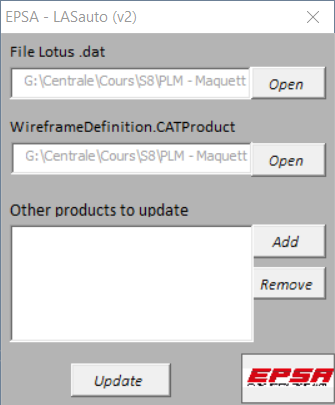
\includegraphics[height=10cm]{img/interface.png}
    \captionof{figure}{Représentation schématique (gauche) et réalisation de l'interface (droite) de l'interface de la Macro}
    \label{fig:interfaceGraphique}
\end{minipage}

\\

\par La fig. \ref{fig:interfaceGraphique} présente la structure souhaitée pour l'interface de la Macro: trois sections se définissent.
\par Premièrement, on retrouve le champ pour la sélection du fichier Lotus \texttt{.dat} avec l'enregistrement de l'analyse cinématique.
\par Deuxièmement, on trouve le champ pour la sélection du Produit Catia pour la définition du filaire à partir des points. La macro va automatiquement repérer à l'intérieur de ce Produit la pièce \texttt{LotusPoints.CATPart} afin de mettre à jour les points. 
\par Troisièmement, on retrouve une section pour la sélection multiple des produits à mettre à jour suite au changement des points LAS : le choix est fait par l'utilisateur en fonction du travail demandé.

\par On remarque que l'utilisateur peut ne pas avoir besoin de changer tous les fichiers chaque fois puisque seulement le fichier \texttt{Lotus.dat} est sensé varier. On souhaiterait donc que cette application garde en mémoire les adresses des fichiers utilisés lors de la dernière utilisation tout en laissant à l'utilisateur la possibilité de les modifier en cas de besoin. Pour ce faire, un nouveau fichier \texttt{params.txt} est créé et mis à jour dans le même répertoire de stockage de la bibliothèque de la macro.

\par On remarque également que le bouton "Cancel" prévu dans la maquette de l'interface se matérialise dans le bouton de fermeture de la fenêtre de la macro.


\subsection{Enregistrement des dernières positions des fichiers} % ---------------------------------

\par Afin de simplifier l'utilisation de la macro, on décide de stocker la dernière valeur de la position du dernier fichier \texttt{WireframeDefinition.CATProduct} dans la première ligne du fichier \texttt{params.txt} et de laisser à l'utilisateur la possibilité de changer cette position à travers l'interface graphique. On implémentera la même solution pour l'ensemble des produits que l'utilisateur ajoutera dans le champ \textit{Other products to update} de l'interface graphique et également pour le dernier fichier Lotus utilisé, afin de pouvoir les charger la fois suivante à l'ouverture de la macro.

\par Afin de charger ces paramètres lors du lancement de l'application, on utilise la subroutine \texttt{UserForm\_Activate} et on implémente une simple lecture du fichier texte params.txt avec un objet de type \textit{TextStream}. Pour l'enregistrement des positions des fichiers avant la fermeture de l'application, on utilise la subroutine \textit{UserForm\_QueryClose} et on remplace tout simplement les nouvelles positions dans le fichier texte. La structure du fichier \texttt{params.txt} se définit donc de façon simple:
\begin{enumerate}
    \item path du dernier fichier \texttt{WireframeDefinition.CATProduct} dans la première ligne
    \item path du dernier fichier Lotus \texttt{.dat} dans la deuxième ligne
    \item path des derniers produits supplémentaires à mettre à jour à partir de la troisième ligne
\end{enumerate}

\par Ainsi, afin de n'écrire qu'une fois dans le fichier params.txt, étant donné que la manipulation d'un fichier txt en VBA est plutôt lourde, nous passons par l'intermédiaire d'un tableau, appelé \textit{update\_products} dans notre code,  tableau dans lequel nous ajoutons ou enlevons le path des produits ainsi ajoutés ou enlevés. Ensuite, nous copions termes à termes les paths dans params.txt à la fermeture de l'UserForm.

\subsection{Messages d'erreurs} % ---------------------------------------------------

\par Différentes erreurs sont pris en compte lors par cette Macro :

\begin{itemize}
    \item Si l'utilisateur oublie de renseigner la path d'un fichier Lotus et clique sur Update, la macro l'oblige à en choisir un
    \item Même méthode s'il oublie de choisir le path de \texttt{WireframeDefinition.CATProduct}.
\end{itemize}

\section{Exemple d'utilisation: voiture de la saison 2020}

% on ne refait toute la voiture --> passation 1As
\par On présente ici une application de la Macro afin de tester son bon fonctionnement et de montrer la démarche typique pour son utilisation au sein de l'EPSA. Cet exemple servira également à aider à l'évaluation de ce projet. Seulement une partie du train avant gauche est présentée par la suite : la reconstruction de l'assemblage complet aurait demandé trop de temps. 

\subsection{Création des pièces filaires} % --------

\par Dans un premier temps, il est nécessaire de créer les pièces filaires dans  \texttt{WireframeDefinition. CATProduct} en utilisant les points à l'intérieur de \texttt{LotusPoints.CATPart}. Ci-dessous une liste complète des filaires à créer, présent dans la Fig. \ref{fig:desk_wireframe_definition} avec une capture d'écran du \textit{Bureau} CATIA permettant de comprendre l'architecture de notre Produit.\footnote{afin d'obtenir la bonne structure, il est conseillé de cacher tout les dossiers "éléments de référence" dans l'arbre et de ne jamais sélectionner les éléments depuis l'affichage de la maquette mais de cliquer directement les éléments dans l'arbre du produit}
\begin{itemize}
    \item Châssis (frame)
    \item Triangles
    \item Biellettes de suspension, de direction et pince
    \item Basculeurs
    \item Barres anti-roulis \footnote{ces filaires n'apparaissent pas à l'heure actuelle mais peuvent être mis en place très facilement dans le \texttt{WireframeDefinition} }
    \item Colonne de direction
    \item Roues
\end{itemize}

\begin{figure}[H]
    \centering
    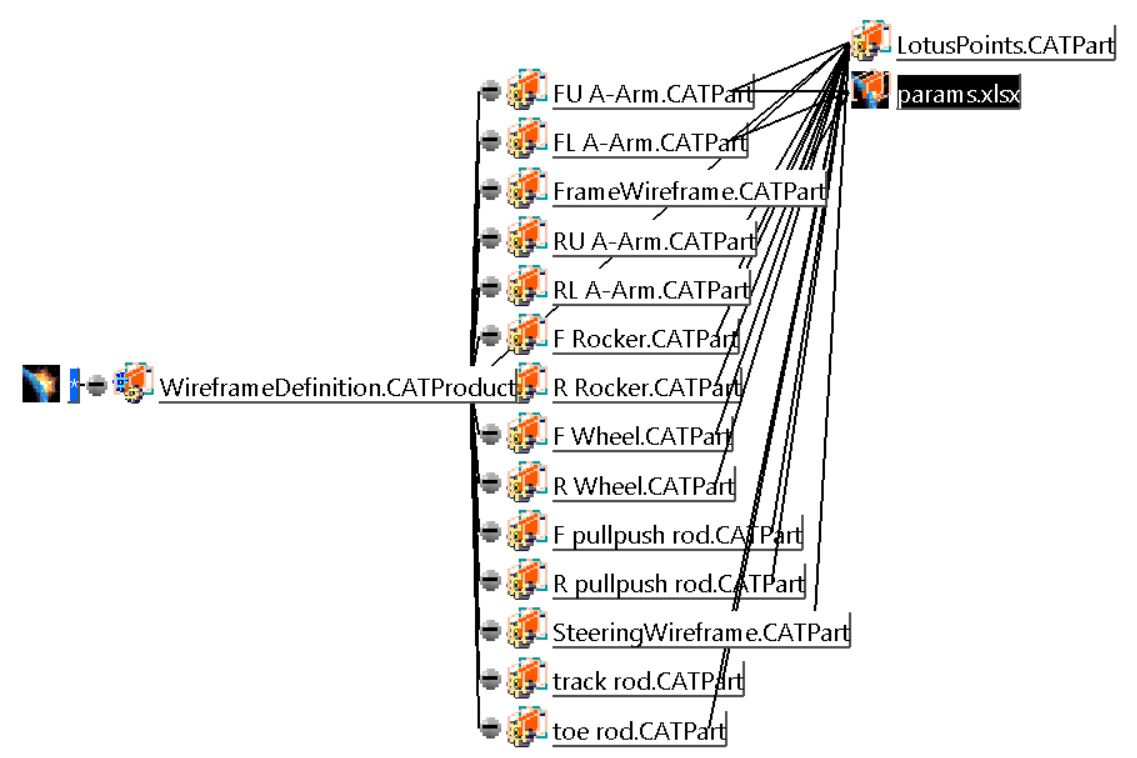
\includegraphics[height=9cm]{img/Desk_wireframe_definition.JPG}
    \caption{Capture du \textit{Bureau} de \texttt{Wireframe\_Definition.CATProduct}, montrant une structure similaire à la Figure \ref{fig:idea}}
    \label{fig:desk_wireframe_definition}
\end{figure}

% exemple de filaire type : triangles
\par Nous remarquons que dans cette étape, l'utilisateur peut définir une orientation personnalisée des repères des pièces. Cela est très utile en phase de conception détaillé afin d'avoir des produits bien faits par rapport aux directions principales du véhicule. En effet, les axes du repère Lotus sont associés à différents grandeurs caractéristiques de la dynamique du véhicule et il est par conséquent impératif que les assemblages soient bien orientés.

\subsection{Création des produits pour la conception détaillée} % ----------------

\par Dans un deuxième temps, on s'occupe de la création des fichiers pour la conception détaillée des pièces. Pour ce faire, on place, à la racine de chacun de ces produits, la pièce filaire correspondante et on la fixe avec une contrainte de fixation. Au fur et au mesure que l'on ajoute des pièces dans les produits, nous conseillons de suivre les règles suivantes:
\begin{itemize}
    \item tout positionnement de pièce à l'intérieur d'un produit de conception détaillée doit se faire par rapport à la pièce filaire à la racine du produit
    \item ranger les contraintes de chaque pièce dans un sous-dossier et cacher l'affichage graphique des contraintes 
\end{itemize}{}
\par Tout le long de la conception détaillée, on peut définir un fichier de paramètres de conception \texttt{params.xlsx} qui permettra à l'utilisateur de stocker de façon méthodique tous les paramètres inter-corrélés à l'intérieur des différents produits. Il s'agit de paramètres comme l'espacement des basculeurs ou le décalages des tubes des triangles par rapport au centre de la rotule : ces valeurs ont la caractéristique de changer très souvent pendant la période de conception du véhicule. L'exemple d'un triangle de suspension est présenté en Fig. \ref{fig:assemblage_tri}.

\begin{figure}
    \centering
    \begin{subfigure}{.5\textwidth}
        \centering
        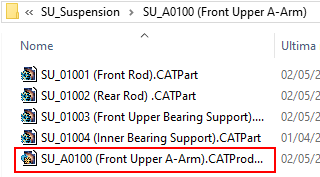
\includegraphics[width=\textwidth]{img/tria_file.png}
        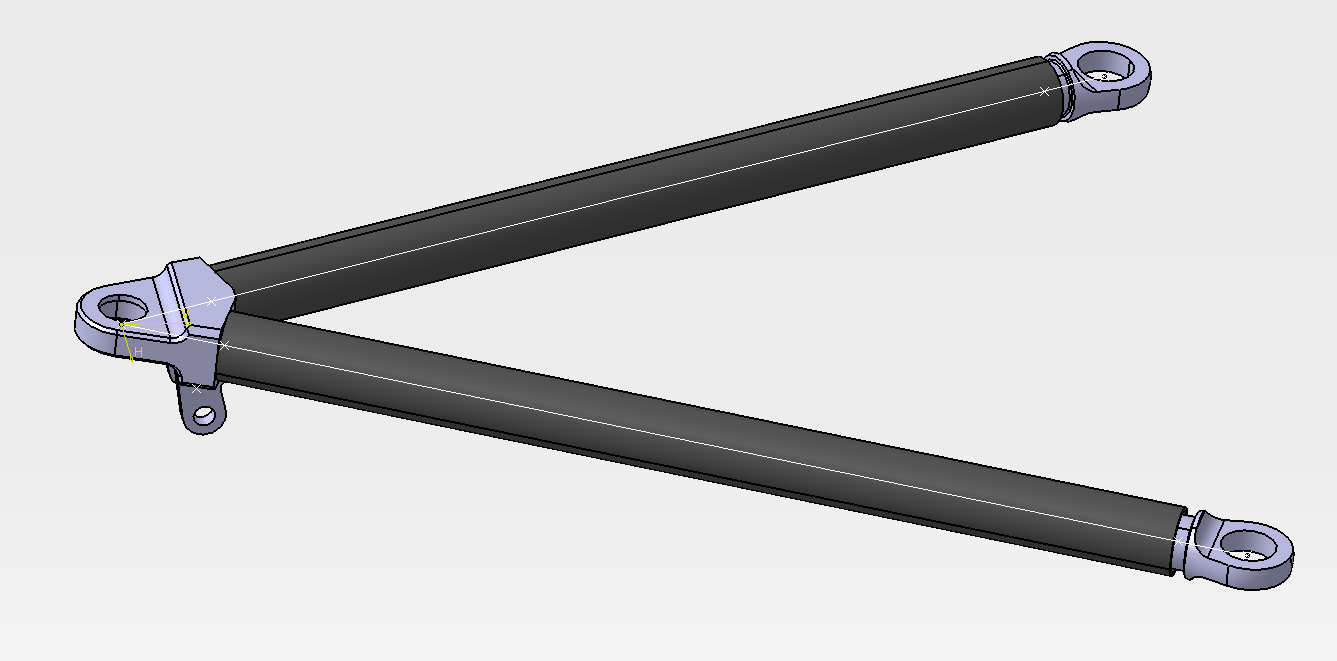
\includegraphics[width=\textwidth]{img/tria_screen.png}
    \end{subfigure}{}
    \begin{subfigure}{.25\textwidth}
        \centering
        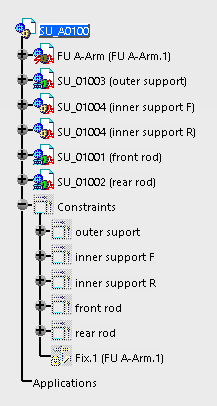
\includegraphics[width=\textwidth]{img/tria_tree.png}
    \end{subfigure}{}
    \caption{Capture d'écran du produit pour la conception détaillée du triangle avant haut gauche}
    \label{fig:assemblage_tri}
\end{figure} % image triangle détaillée

\subsection{Création d'un assemblage global pour la Liaison au Sol} % -----------------

\par Enfin, nous ajoutons les produits de conception détaillée à l'intérieur d'un assemblage général pour la totalité du système de Liaison au Sol du véhicule (Fig. \ref{fig:assemblage_las}). Pour ce faire, on place en fixation globale le produit détaillé du châssis et on accroche graduellement tous les produits détaillés.

% explication des liaisons paramétrées pour l'étude des collisions
\par Afin de pouvoir étudier le mouvement et les collisions éventuelles entre les différentes organes du véhicule, certaines  liaisons peuvent être paramétrées au niveau de l'assemblage \texttt{Suspension.CATProduct} : c'est l'exemple du débattement de l'amortisseur (paramètre \texttt{FL offset}) dans l'arbre du produit.

% explication des système e mesure pour controler les dimension critiques 
De même, certaines grandeurs caractéristiques (comme par exemple la voie et empattement) pourront être implémentées comme applications de type \textit{mesure} dans l'arbre de ce produit global afin de pouvoir surveiller leur valeur tout le long de la conception. 

\begin{figure}
    \centering
    \begin{subfigure}{.5\textwidth}
        \centering
        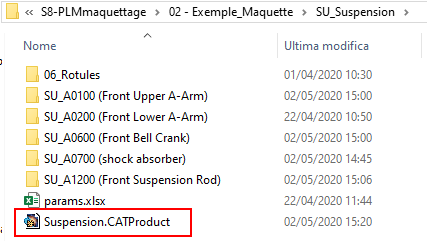
\includegraphics[width=\textwidth]{img/susp_file.png}
        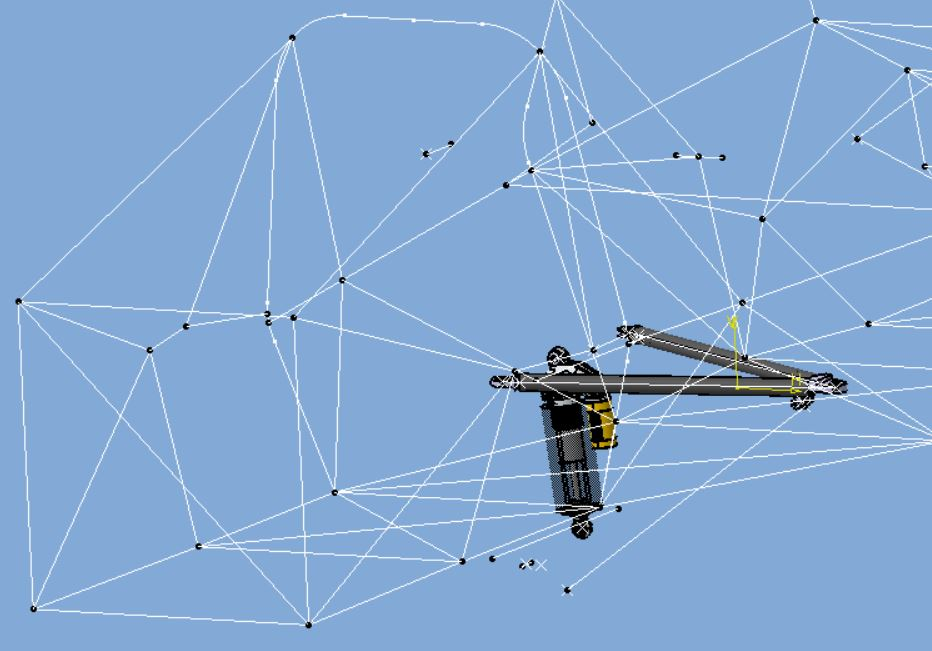
\includegraphics[width=\textwidth]{img/susp_screen.JPG}
    \end{subfigure}{}
    \begin{subfigure}{.25\textwidth}
        \centering
        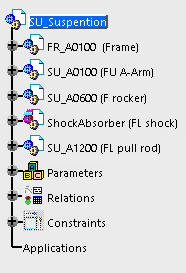
\includegraphics[width=\textwidth]{img/susp_tree.png}
    \end{subfigure}{}
    \caption{Capture d'écran de l'Assemblage LAS qui est mis à jour par la macro}
    \label{fig:assemblage_las}
\end{figure} % image suspension 

\subsection{Une proposition pour l'assemblage châssis} %-------------------------

\par Afin de démontrer la versatilité de l'architecture choisie, il est également possible d'insérer dans des assemblages d'autres sous-systèmes, certains filaires de la LAS. 
En effet, un véhicule comprend de nombreuses interactions, et la prise en compte de ces interfaces fonctionnelles est primordiale.

\par Nous proposons donc le placement du filaire des triangles de suspension et de la colonne de direction dans celui du châssis. Ces filaires seront mis à jour par la macro.

\subsection{Mise en application}

Voici les étapes à suivre pour tester la Macro, un exemple est donné en Fig. \ref{fig:maj_assy}
\begin{enumerate}
    \item Installez la macro comme spécifié dans le guide d'installation, présent dans la section \ref{install_macro}.
    \item Lancez la macro comme indiqué dans ce même guide.
    \item Sélectionnez le fichier Lotus \texttt{Test1.dat}, rangé dans le dossier \textit{04 - Tests}
    \item Sélectionnez le produit \texttt{WireframeDefinition}, dans le dossier \textit{02 - Exemple\_Maquette > wireframe}
    \item Ajoutez les produits que vous souhaitez mettre à jour dans le dossier \textit{02 - Exemple\_Maquette}, par exemple le fichier \texttt{SU\_A0100 (Front Uper A-Arm).CATProduct}
    \item Mettez à jour. Vous aurez normalement des messages d'informations sur le contenu de la mise à jour.
    \item Fermez la macro et observez l'assemblage \texttt{Suspension}
    \item Relancez la macro et répétez les étapes précédentes la concernant, en choisissant cette fois ci le fichier \texttt{Test2.dat} dans le dossier \textit{04 - Tests}. Vous devriez voir notamment que vos choix précédents ont été mis en mémoire par la macro et que vous n'aurez pas à sélectionner à nouveau \texttt{WireframeDefinition.CATProduct} et \texttt{Suspension.CATProduct}.
    \item Mettez à jour et observez l'assemblage \texttt{Suspension}. Vous pourrez noter que l'architecture a bel et bien été mis à jour.
\end{enumerate}

\begin{figure}
    \centering
    \begin{subfigure}{.35\textwidth}
        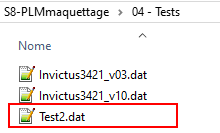
\includegraphics[width=.8\textwidth]{img/maj_file1.png}
        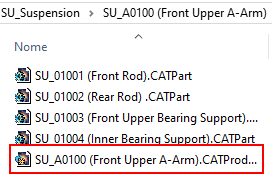
\includegraphics[width=\textwidth]{img/maj_file3.png}
    \end{subfigure}{}
    \begin{subfigure}{.3\textwidth}
        \centering
        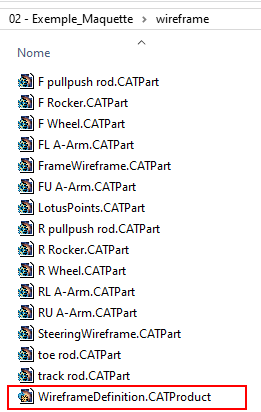
\includegraphics[width=\textwidth]{img/maj_file2.png}
    \end{subfigure}{}
    \begin{subfigure}{.3\textwidth}
        \centering
        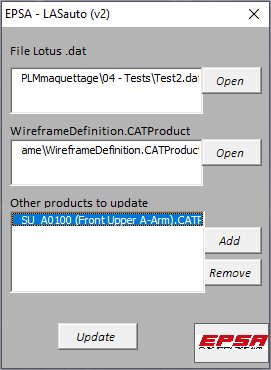
\includegraphics[width=\textwidth]{img/maj_screen.png}
    \end{subfigure}{}
    \caption{exemple de test de la macro}
    \label{fig:maj_assy}
\end{figure} % capture d'écran mise en application 
\section{Conclusion}


Le but de ce projet était donc de permettre la mise à jour simple et rapide d'un Assemblage Catia portant sur une liaison au sol, dimensionnée cinématiquement sur un logiciel annexe nommé Lotus.
En passant par de la programmation VBA, ce résultat est rempli et permet à l'utilisateur une utilisation ergonomique, à l'aide d'un UserForm simple et épurée.
La programmation VBA et les fonctionnalités que nous avons incorporé permettent une automatisation, une répétabilité et une versatilité conséquente.
Vous trouverez ci-dessous les innovations futures de \textit{LASAuto}, que nous n'avons pas pu implémenter :

\paragraph{Développements futurs}
\begin{itemize}
    \item Mise en parallèle avec le modèle Mécamaster.
    \item Symétrie de la voiture (qui n'est pas symétrique cf. Ackermann).
    \item Enlever les centres de gravité dans Lotus.
    \item Enlever les bugs qui apparaissent lorsqu'un Product ne veut pas se mettre à jour.
\end{itemize}


 

%-------------- annexe -----------------------
\appendix
\section{Annexe}


\subsection{Paramétrage CATIA pour les références entre pièces} %----------------------

\par La fig. \ref{fig:paramCatia} présente les options à cocher afin d'avoir une bonne transmission des références entre les pièces des assemblages.

\hfigure{img/parametrageCatia.png}{width=\linewidth}{
Préférences Catia conseillées
}{paramCatia}

\subsection{Installation de la Macro}
\label{install_macro}
%-------------------------------------------------------

\par Vous trouverez, dans les pages suivantes, la démarche nécessaire afin d'installer la macro dans le répertoire de travail de la suspension d'un nouveau véhicule.

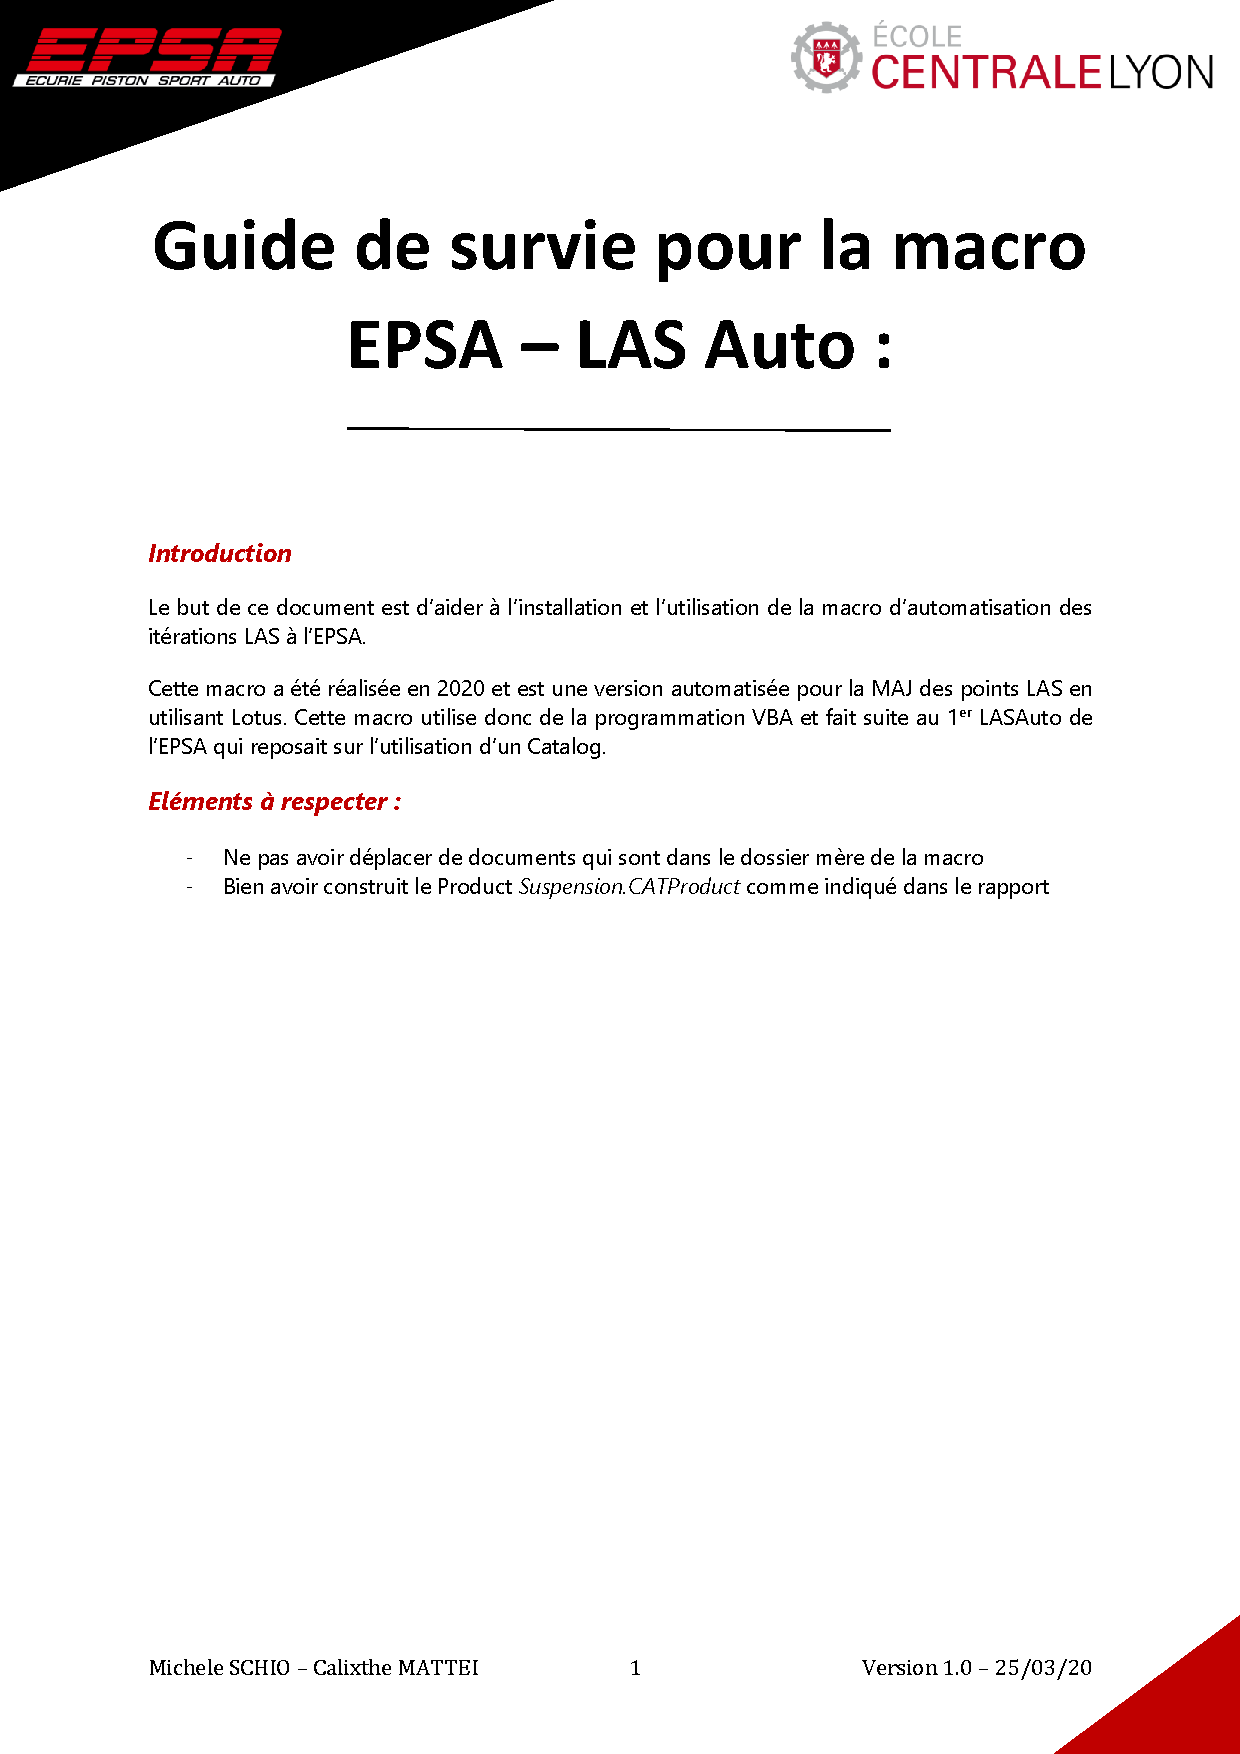
\includepdf[pages=-]{img/tuto_installation.pdf}








\end{document}
